% ============================================================================
%  Supporting Information template (chemistry)
%  Compile separately:  pdflatex si.tex
% ============================================================================
\documentclass[12pt,a4paper]{article}
\usepackage[utf8]{inputenc}
\usepackage[T1]{fontenc}
\usepackage{mathptmx}   % Times-like (universally available in TeX Live)
\usepackage[margin=2.5cm]{geometry}
\usepackage{graphicx}
\graphicspath{{figures/}}
\usepackage{booktabs}
\usepackage[version=4]{mhchem}
\usepackage{siunitx}
\usepackage[font=small,labelfont=bf]{caption}
\usepackage[colorlinks=true]{hyperref}

\title{Supporting Information\\[6pt] \large Title of the Manuscript: Subtitle}
\author{First Author, Second Author, Corresponding Author*\\
  Department of Chemistry, Indian Institute of Science Education and Research
  Bhopal, Bhopal Bypass Road, Bhauri, Bhopal 462066, MP, India.\\
  *E-mail: corresponding@iiserb.ac.in}
\date{}

\begin{document}
\maketitle
\thispagestyle{empty}

% Mini TOC (RSC/ACS practice)
\section*{Contents}
\begin{itemize}
  \item General experimental methods (pages S2--S3)
  \item Synthetic procedures (pages S3--S6)
  \item \ce{^1H} and \ce{^{13}C} NMR spectra, compounds \textbf{1}--\textbf{9} (pages S7--S16)
  \item HRMS spectra (pages S17--S21)
  \item Crystallographic data and checkCIF reports (pages S22--S28)
  \item Computational details and Cartesian coordinates (pages S29--S34)
\end{itemize}

\newpage
\section{General experimental methods}
All manipulations were performed under a nitrogen atmosphere using standard
Schlenk techniques unless otherwise stated. \ldots{}

\section{Synthetic procedures}
\subsection{Compound \textbf{1}}
\ldots{}

\section{NMR spectra}
\begin{figure}[htbp]
\centering
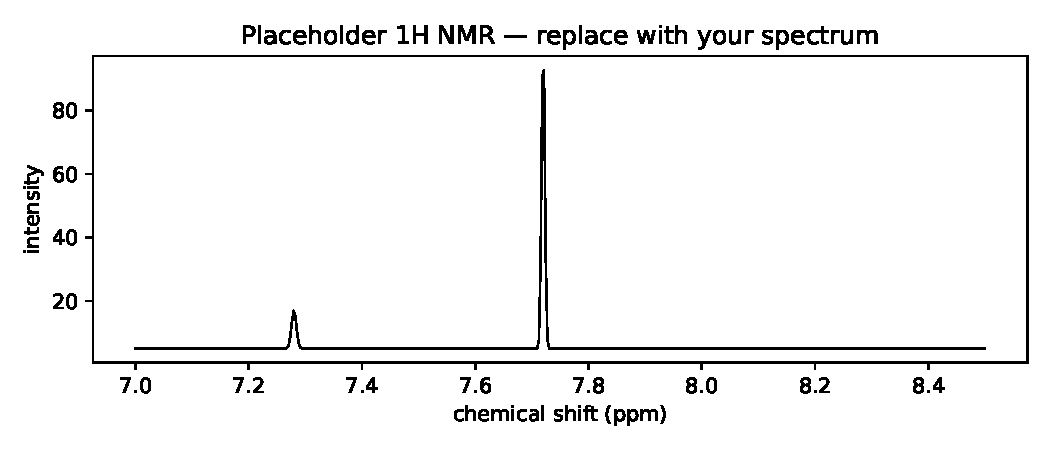
\includegraphics[width=0.9\linewidth]{nmr_1h_compound1.pdf}
\caption{\ce{^1H} NMR spectrum of compound \textbf{1} (\SI{400}{\mega\hertz},
\ce{CDCl3}, \SI{298}{\kelvin}).}
\label{fig:s1}
\end{figure}

\end{document}
